\documentclass[preprint,12pt,aps,pra,showkeys,amsmath,amssymb,superscriptaddress,floatfix]{revtex4-2}
\usepackage[T1]{fontenc}
\usepackage[utf8]{inputenc}
\usepackage{amsmath,amssymb,amsthm,mathtools,mathrsfs}
\usepackage{microtype,booktabs,enumitem}
\usepackage{xcolor,tikz,etoolbox}
\usepackage[skins,breakable]{tcolorbox}
\usepackage{needspace}
% Keep diagram geometry independent of REVTeX preprint body spacing.
\AtBeginEnvironment{tikzpicture}{\linespread{1}\selectfont}
\usetikzlibrary{arrows.meta,positioning,calc,fit,decorations.pathreplacing}
\usepackage{graphicx}
\usepackage{hyperref}

\definecolor{MMBlue}{RGB}{0,82,155}
\definecolor{MMOrange}{RGB}{200,80,0}
\tikzset{
 mmnode/.style={draw=MMBlue,rounded corners=2pt,fill=MMBlue!4,align=left,execute at begin node={\raggedright},text width=5cm,font=\fontsize{10}{12}\selectfont,inner sep=6pt},
 mmimport/.style={mmnode,draw=black!65,fill=black!4},
 mmcandidate/.style={mmnode,draw=MMOrange,dashed,fill=MMOrange!5},
 mmrejected/.style={mmnode,draw=black,densely dotted,fill=black!8},
 mmproof/.style={->,thick,MMBlue},
 mmflow/.style={->,semithick,black!70},
 mmrepair/.style={->,dashed,thick,MMOrange},
 mmcandidatearrow/.style={->,dashed,semithick,MMOrange},
 mmnote/.style={font=\scriptsize,fill=white,inner sep=2pt,align=center}}

\usepackage[section]{placeins}
\setlength{\emergencystretch}{3em}
\setlist{itemsep=3pt,topsep=4pt}
\newtheorem{theorem}{Theorem}[section]
\newtheorem{proposition}[theorem]{Proposition}
\newtheorem{lemma}[theorem]{Lemma}
\newtheorem{corollary}[theorem]{Corollary}
\theoremstyle{definition}
\newtheorem{definition}[theorem]{Definition}
\newtheorem{example}[theorem]{Example}
\theoremstyle{remark}
\newtheorem{remark}[theorem]{Remark}
% Avoid isolated statement headings and single-line paragraph fragments.
\BeforeBeginEnvironment{theorem}{\Needspace{6\baselineskip}}
\BeforeBeginEnvironment{definition}{\Needspace{5\baselineskip}}
\BeforeBeginEnvironment{proposition}{\Needspace{5\baselineskip}}
\BeforeBeginEnvironment{lemma}{\Needspace{5\baselineskip}}
\BeforeBeginEnvironment{corollary}{\Needspace{5\baselineskip}}
\clubpenalty=5000
\widowpenalty=5000
\newcommand{\R}{\mathbb R}\newcommand{\Z}{\mathbb Z}\newcommand{\N}{\mathbb N}
\newcommand{\Pa}{\operatorname{Pa}}\newcommand{\Desc}{\operatorname{Desc}}
\newcommand{\cl}{\operatorname{cl}}\newcommand{\cost}{\operatorname{cost}}
\newcommand{\status}{\operatorname{status}}
% Faculty cards: a visual rail groups the five faculties within one agent.
% The rail has no arrowhead and does not represent a proof dependency.
\newcommand{\mmfacultybadge}[1]{%
 \node[circle,draw=MMBlue,line width=1pt,fill=white,
 minimum size=7mm,inner sep=0pt,font=\sffamily\small\bfseries,text=MMBlue]
 at ([xshift=15pt,yshift=-15pt]frame.north west) {#1};}
\newcommand{\mmfacultyrail}{%
 \draw[MMBlue!80,line width=1pt]
 ([xshift=15pt,yshift=2pt]frame.north west)--
 ([xshift=15pt,yshift=-2pt]frame.south west);}
\newtcolorbox{mmfacultybox}[2]{enhanced,breakable,
 colback=MMBlue!4,colframe=MMBlue!4,boxrule=0pt,arc=3pt,
 left=39pt,right=9pt,top=7pt,bottom=7pt,
 before skip=2pt,after skip=2pt,
 fontupper=\normalsize\linespread{1.15}\selectfont,
 overlay unbroken={\mmfacultyrail\mmfacultybadge{#1}},
 overlay first={\mmfacultyrail\mmfacultybadge{#1}},
 overlay middle={\mmfacultyrail},overlay last={\mmfacultyrail}}
\newcommand{\mmfaculty}[3]{%
 \begin{mmfacultybox}{#1}{#2}
 {\sffamily\bfseries\color{MMBlue}#2}\par\smallskip #3
 \end{mmfacultybox}}
\newcommand{\agent}[9]{%
 \Needspace{8\baselineskip}
 \subsubsection{#1}
 \noindent\textbf{Object.} #2\par
 \noindent\textbf{Role.} #3\par\smallskip
 \mmfaculty{E}{Ego}{#4}
 \mmfaculty{M}{Memory}{#5}
 \mmfaculty{I}{Intellect}{#6}
 \mmfaculty{S}{Sense}{#7}
 \mmfaculty{A}{Action}{#8}
 \smallskip\noindent #9\par}

\usepackage{longtable,array}
\providecommand{\tightlist}{\setlength{\itemsep}{2pt}\setlength{\parskip}{0pt}}
% Keep short report abstracts with their title instead of REVTeX's optional preprint break.
\makeatletter
\def\frontmatter@abstract@produce{\par\addvspace{\frontmatter@preabstractspace}%
\begingroup\prep@absbox\unvbox\absbox\post@absbox\endgroup
\addvspace{\frontmatter@postabstractspace}}
\makeatother
\newcommand{\field}[2]{\par\smallskip\noindent\textbf{#1.} #2\par}
\newcommand{\reportcaption}[1]{\par\smallskip{\small\noindent #1\par}}


\hypersetup{colorlinks=true,linkcolor=MMBlue,urlcolor=MMBlue,pdftitle={Euclidean Algorithm and Bézout's Identity},pdfauthor={Dibakar Sigdel}}

\begin{document}

\title{Euclidean Algorithm and Bézout's Identity\\[4pt]\large An End-to-End Meta-Math Walkthrough}

\author{Dibakar Sigdel}

\affiliation{Mindverse Computing LLC, Lynnwood, WA 98087, USA}

\date{October 2026}

\begin{abstract}

A decreasing remainder sequence proves termination; a second invariant
carries a certificate in the original signed inputs. Their convergence
identifies the positive gcd and supplies modular inverses. This report
presents a complete proof relative to explicit imports, a dependency
graph, versioned node contracts, five-faculty activities, exact
examples, and an illustrative repair. The interactions are authored
explanations, not a transcript of deployed agents or a proof-assistant
certificate.

\end{abstract}

\maketitle

\linespread{1.12}\selectfont

\noindent\textbf{Project NT-01 \quad Report version 1 \quad Number Theory}

\section{Target and import contract}

\begin{theorem}

For every \(a,b\in\mathbb Z\) with \((a,b)\ne(0,0)\), the extended
Euclidean algorithm terminates and returns integers \(d,u,v\) such that
\(d=\gcd(a,b)>0\) and \(au+bv=d\). For every \(m\ge2\), an integer \(a\)
is invertible modulo \(m\) if and only if \(\gcd(a,m)=1\).

\end{theorem}

\subsection{Foundations and permitted imports}

\begin{enumerate}
\def\labelenumi{\arabic{enumi}.}
\item
  Divisibility means \(c\mid x\) if \(x=ck\) for an integer \(k\). The
  gcd is the largest positive common divisor; positive common divisors
  form a nonempty finite set when the inputs are not both zero.
\item
  Division with remainder: for \(A\ge0\) and \(B>0\), unique integers
  \(q,r\) satisfy \(A=qB+r\) and \(0\le r<B\). Well-ordering rules out
  an infinite strictly decreasing sequence of positive integers.
\item
  Congruence \(x\equiv y\pmod m\) means \(m\mid(x-y)\). No Bézout
  theorem, Euclid lemma, or unique factorization is imported.
\end{enumerate}

\clearpage\section{Node interaction workflow}

\begin{center}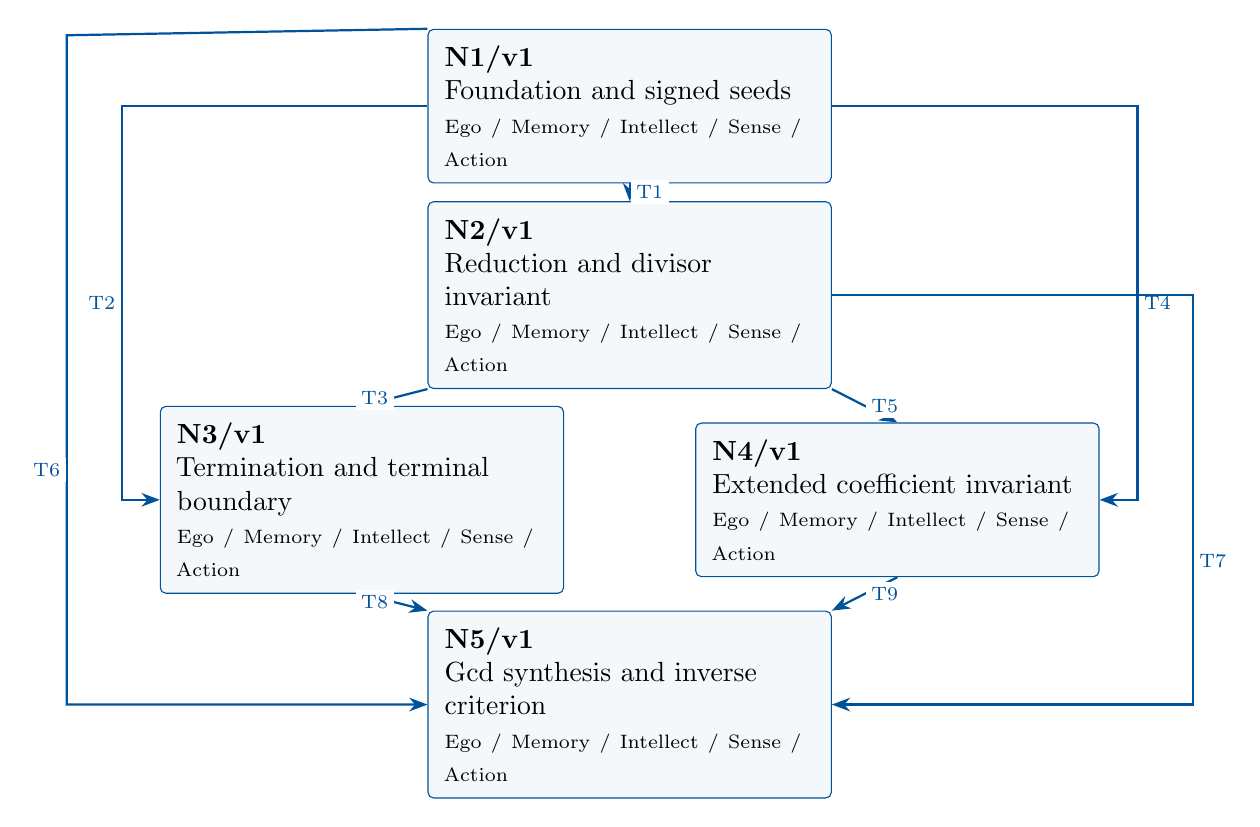
\begin{tikzpicture}[>=Stealth,x=1cm,y=1cm]

\node[mmnode,text width=4.7cm,minimum height=1.35cm] (N1) at (0,0) {\textbf{N1/v1}\\Foundation and signed seeds\\{\scriptsize Ego / Memory / Intellect / Sense / Action}};

\node[mmnode,text width=4.7cm,minimum height=1.35cm] (N2) at (0,-2.4) {\textbf{N2/v1}\\Reduction and divisor invariant\\{\scriptsize Ego / Memory / Intellect / Sense / Action}};

\node[mmnode,text width=4.7cm,minimum height=1.35cm] (N3) at (-3.4,-5.0) {\textbf{N3/v1}\\Termination and terminal boundary\\{\scriptsize Ego / Memory / Intellect / Sense / Action}};

\node[mmnode,text width=4.7cm,minimum height=1.35cm] (N4) at (3.4,-5.0) {\textbf{N4/v1}\\Extended coefficient invariant\\{\scriptsize Ego / Memory / Intellect / Sense / Action}};

\node[mmnode,text width=4.7cm,minimum height=1.35cm] (N5) at (0,-7.6) {\textbf{N5/v1}\\Gcd synthesis and inverse criterion\\{\scriptsize Ego / Memory / Intellect / Sense / Action}};

\draw[mmproof] (N1.south) -- node[mmnote,right] {T1} (N2.north);

\draw[mmproof] (N1.west) -- (-6.45,0) -- node[mmnote,left] {T2} (-6.45,-5) -- (N3.west);

\draw[mmproof] (N2.south west) -- node[mmnote,left] {T3} (N3.north);

\draw[mmproof] (N1.east) -- (6.45,0) -- node[mmnote,right] {T4} (6.45,-5) -- (N4.east);

\draw[mmproof] (N2.south east) -- node[mmnote,right] {T5} (N4.north);

\draw[mmproof] (N1.north west) -- (-7.15,.9) -- node[mmnote,left,pos=.65] {T6} (-7.15,-7.6) -- (N5.west);

\draw[mmproof] (N2.east) -- (7.15,-2.4) -- node[mmnote,right,pos=.65] {T7} (7.15,-7.6) -- (N5.east);

\draw[mmproof] (N3.south) -- node[mmnote,left] {T8} (N5.north west);

\draw[mmproof] (N4.south) -- node[mmnote,right] {T9} (N5.north east);

\end{tikzpicture}\end{center}

\reportcaption{Blue arrows are accepted mathematical dependencies, with exact transfers T1--T9 below. Repair messages are described separately; they are not premises of the proof.}

\subsection{Execution loop associated with the proof}
The repeated computation is an execution loop, not a cycle of proof premises.
All right-hand sides in the final assignment use the old state.
\begingroup\small\linespread{1.0}\selectfont
\begin{verbatim}
require integer a, b, not both zero
A, B = abs(a), abs(b)
sA, tA = sign(a), 0
sB, tB = 0, sign(b)
while B != 0:
    q, r = divmod(A, B)
    nextS, nextT = sA - q*sB, tA - q*tB
    assert 0 <= r < B and A == q*B + r
    assert r == nextS*a + nextT*b
    A, B, sA, tA, sB, tB = B, r, sB, tB, nextS, nextT
return A, sA, tA
\end{verbatim}
\endgroup

\clearpage\subsection{Versioned evidence-transfer ledger}

\begingroup\small\linespread{1.05}\selectfont\renewcommand{\field}[2]{\par\noindent\textbf{#1.} #2\par}

\Needspace{5\baselineskip}\smallskip\noindent\textbf{T1: N1/E1 v1 to N2.1}

\field{Claim}{\(r_0=|a|\), \(r_1=|b|\) have the same common divisors as \(a,b\);
\(r_i=s_i a+t_i b\) for \(i=0,1\).}

\field{Compatibility}{Normalized nonnegative pair; division still requires a positive second
entry.}

\field{Evidence}{Node N1 activities below and the continuous proof in Section~\ref{sec:proof}.}

\Needspace{5\baselineskip}\smallskip\noindent\textbf{T2: N1/E1 v1 to N3.3}

\field{Claim}{\(r_0=|a|\), \(r_1=|b|\) have the same common divisors as \(a,b\);
\(r_i=s_i a+t_i b\) for \(i=0,1\).}

\field{Compatibility}{The original pair is not both zero.}

\field{Evidence}{Node N1 activities below and the continuous proof in Section~\ref{sec:proof}.}

\Needspace{5\baselineskip}\smallskip\noindent\textbf{T3: N2/E2 v1 to N3.1}

\field{Claim}{\(A=qB+r\), \(0\le r<B\), and the pairs \((A,B)\) and \((B,r)\) have
identical positive common divisors.}

\field{Compatibility}{The next divisor is strictly smaller whenever the run continues.}

\field{Evidence}{Node N2 activities below and the continuous proof in Section~\ref{sec:proof}.}

\Needspace{5\baselineskip}\smallskip\noindent\textbf{T4: N1/E1 v1 to N4.3}

\field{Claim}{\(r_0=|a|\), \(r_1=|b|\) have the same common divisors as \(a,b\);
\(r_i=s_i a+t_i b\) for \(i=0,1\).}

\field{Compatibility}{Both seed coefficient identities hold.}

\field{Evidence}{Node N1 activities below and the continuous proof in Section~\ref{sec:proof}.}

\Needspace{5\baselineskip}\smallskip\noindent\textbf{T5: N2/E2 v1 to N4.1}

\field{Claim}{\(A=qB+r\), \(0\le r<B\), and the pairs \((A,B)\) and \((B,r)\) have
identical positive common divisors.}

\field{Compatibility}{Use the very same quotients as the remainder run.}

\field{Evidence}{Node N2 activities below and the continuous proof in Section~\ref{sec:proof}.}

\Needspace{5\baselineskip}\smallskip\noindent\textbf{T6: N1/E1 v1 to N5.1}

\field{Claim}{\(r_0=|a|\), \(r_1=|b|\) have the same common divisors as \(a,b\);
\(r_i=s_i a+t_i b\) for \(i=0,1\).}

\field{Compatibility}{The original signed inputs have the normalized divisor set.}

\field{Evidence}{Node N1 activities below and the continuous proof in Section~\ref{sec:proof}.}

\Needspace{5\baselineskip}\smallskip\noindent\textbf{T7: N2/E2 v1 to N5.1}

\field{Claim}{\(A=qB+r\), \(0\le r<B\), and the pairs \((A,B)\) and \((B,r)\) have
identical positive common divisors.}

\field{Compatibility}{Divisor-set preservation holds through every valid step.}

\field{Evidence}{Node N2 activities below and the continuous proof in Section~\ref{sec:proof}.}

\Needspace{5\baselineskip}\smallskip\noindent\textbf{T8: N3/E3 v1 to N5.1}

\field{Claim}{Every valid run reaches \((d,0)\) after finitely many divisions, with
\(d>0\).}

\field{Compatibility}{A finite positive terminal remainder exists.}

\field{Evidence}{Node N3 activities below and the continuous proof in Section~\ref{sec:proof}.}

\Needspace{5\baselineskip}\smallskip\noindent\textbf{T9: N4/E4 v1 to N5.2}

\field{Claim}{Every generated remainder satisfies \(r_j=s_ja+t_jb\) with integer
coefficients.}

\field{Compatibility}{Select coefficients attached to the last nonzero remainder.}

\field{Evidence}{Node N4 activities below and the continuous proof in Section~\ref{sec:proof}.}

\endgroup

\clearpage\section{Agent roles and five-faculty activities}

\subsection{N1/v1: Foundation and signed seeds}

\field{Object and role}{Own the input domain and two initial coefficient identities; enable
later certificates to refer to the original inputs.}

\field{Inputs}{\(a,b\in\mathbb Z\), not both zero.}

\mmfaculty{E}{Ego}{Publish only admissible inputs and signed seed identities; keep the
target gcd positive.}

\mmfaculty{M}{Memory}{Retain the input pair, divisibility, absolute value, and
\(\varepsilon(x)=\operatorname{sgn}(x)\) with \(\varepsilon(0)=0\).}

\mmfaculty{I}{Intellect}{Normalize magnitudes while expressing coefficients in the original
signed integers.}

\mmfaculty{S}{Sense}{Reject \((0,0)\); permit one zero and either input order.}

\mmfaculty{A}{Action}{Set \((r_0,r_1)=(|a|,|b|)\). Continue with the numbered deductions
below, retaining the exact export.}

\smallskip\noindent\textbf{Numbered mathematical activities}

\begin{enumerate}[label=N1.\arabic*,leftmargin=3.4em]

\item Set \((r_0,r_1)=(|a|,|b|)\).

\item Set \((s_0,t_0)=(\varepsilon(a),0)\) and
\((s_1,t_1)=(0,\varepsilon(b))\).

\item Check \(r_0=s_0a+t_0b\) and \(r_1=s_1a+t_1b\); \(c\mid x\) iff
\(c\mid|x|\).

\end{enumerate}

\field{Export E1/v1}{\(r_0=|a|\), \(r_1=|b|\) have the same common divisors as \(a,b\);
\(r_i=s_i a+t_i b\) for \(i=0,1\).}

\field{Acceptance gate}{Both seed identities hold and at least one remainder is positive.}

\field{Targeted repair}{If an input sign changes, regenerate its seed and recheck N4 and N5.}

\clearpage

\subsection{N2/v1: Reduction and divisor invariant}

\field{Object and role}{Own a valid division and the equality of common-divisor sets; supply
both progress and coefficient updates.}

\field{Inputs}{N1/E1; a current pair \(A\ge0\), \(B>0\).}

\mmfaculty{E}{Ego}{Publish preservation for a valid step, without asserting that a complete
run has terminated.}

\mmfaculty{M}{Memory}{Retrieve division with remainder and closure of divisibility under
integer linear combinations.}

\mmfaculty{I}{Intellect}{Prove both containments of the common-divisor sets.}

\mmfaculty{S}{Sense}{Require \(B>0\) before division and audit the strict remainder bound.}

\mmfaculty{A}{Action}{Compute \(A=qB+r\) with \(0\le r<B\). Continue with the numbered
deductions below, retaining the exact export.}

\smallskip\noindent\textbf{Numbered mathematical activities}

\begin{enumerate}[label=N2.\arabic*,leftmargin=3.4em]

\item Compute \(A=qB+r\) with \(0\le r<B\).

\item If \(c\mid A,B\), then \(c\mid A-qB=r\).

\item If \(c\mid B,r\), then \(c\mid qB+r=A\).

\end{enumerate}

\field{Export E2/v1}{\(A=qB+r\), \(0\le r<B\), and the pairs \((A,B)\) and \((B,r)\) have
identical positive common divisors.}

\field{Acceptance gate}{The division equation, remainder bounds, and both divisor implications
are established.}

\field{Targeted repair}{An inadmissible zero divisor routes to the stop condition, not to a
fabricated next remainder; recheck N3--N5.}

\clearpage

\subsection{N3/v1: Termination and terminal boundary}

\field{Object and role}{Own the decreasing integer measure and the positive terminal value.}

\field{Inputs}{N2/E2 and the nonzero-input condition in N1/E1.}

\mmfaculty{E}{Ego}{Export finite termination and positivity, leaving gcd identification to
N5.}

\mmfaculty{M}{Memory}{Retain well-ordering and all remainder inequalities from N2.}

\mmfaculty{I}{Intellect}{Use the current positive divisor as the strictly decreasing measure.}

\mmfaculty{S}{Sense}{Stop when the second entry is zero, including the initial state; do not
require the first quotient to be positive.}

\mmfaculty{A}{Action}{While \(r_j>0\), form \(0\le r_{j+1}<r_j\). Continue with the numbered
deductions below, retaining the exact export.}

\smallskip\noindent\textbf{Numbered mathematical activities}

\begin{enumerate}[label=N3.\arabic*,leftmargin=3.4em]

\item While \(r_j>0\), form \(0\le r_{j+1}<r_j\).

\item An infinite run would be an infinite descent of positive integers.

\item At termination the first entry is positive: it was the last positive
divisor, or the nonzero initial magnitude.

\end{enumerate}

\field{Export E3/v1}{Every valid run reaches \((d,0)\) after finitely many divisions, with
\(d>0\).}

\field{Acceptance gate}{Both immediate termination and a run with divisions end at a positive
first entry and zero second entry.}

\field{Targeted repair}{Replace an incorrect continuation test by \(B\ne0\); invalidate a
proposed extra transition and recheck N5.}

\clearpage

\subsection{N4/v1: Extended coefficient invariant}

\field{Object and role}{Transport each remainder reduction into integer coefficient space.}

\field{Inputs}{N1/E1 seeds and the quotient sequence from N2/E2.}

\mmfaculty{E}{Ego}{Export an identity for each remainder; do not identify a gcd from an
identity alone.}

\mmfaculty{M}{Memory}{Retain both preceding coefficient pairs and their matching remainder
indices.}

\mmfaculty{I}{Intellect}{Apply exactly the same linear recurrence to remainders and their
coefficients.}

\mmfaculty{S}{Sense}{Use the old pairs simultaneously; distinguish the coefficients of the
last nonzero remainder from those of zero.}

\mmfaculty{A}{Action}{Define \(s_{j+1}=s_{j-1}-q_js_j\) and \(t_{j+1}=t_{j-1}-q_jt_j\).
Continue with the numbered deductions below, retaining the exact export.}

\smallskip\noindent\textbf{Numbered mathematical activities}

\begin{enumerate}[label=N4.\arabic*,leftmargin=3.4em]

\item Define \(s_{j+1}=s_{j-1}-q_js_j\) and \(t_{j+1}=t_{j-1}-q_jt_j\).

\item Substitute the two preceding identities into \(r_{j+1}=r_{j-1}-q_jr_j\).

\item Induct from the seed identities to every generated index.

\end{enumerate}

\field{Export E4/v1}{Every generated remainder satisfies \(r_j=s_ja+t_jb\) with integer
coefficients.}

\field{Acceptance gate}{The recurrence preserves \(r_{j+1}=s_{j+1}a+t_{j+1}b\) at every step.}

\field{Targeted repair}{Recompute the first mismatched coefficient pair; downstream pairs and N5
must be rechecked.}

\clearpage

\subsection{N5/v1: Gcd synthesis and inverse criterion}

\field{Object and role}{Join divisor preservation, termination, and the coefficient invariant;
export both directions of the inverse criterion.}

\field{Inputs}{N1--N4 for the same input pair and remainder sequence.}

\mmfaculty{E}{Ego}{Publish the theorem only after positivity, divisibility, maximality, and
the signed certificate are joined.}

\mmfaculty{M}{Memory}{Retrieve the terminal pair, the preserved divisor set, its coefficient
pair, and the definition of congruence.}

\mmfaculty{I}{Intellect}{Identify the divisors of \((d,0)\) and turn a Bézout identity into a
modular inverse.}

\mmfaculty{S}{Sense}{A combination alone does not identify a gcd; check both directions of
the inverse equivalence.}

\mmfaculty{A}{Action}{The common divisors of the original pair equal the positive divisors of
\(d\); thus \(d\mid a,b\) and any common divisor is at most \(d\).
Continue with the numbered deductions below, retaining the exact export.}

\smallskip\noindent\textbf{Numbered mathematical activities}

\begin{enumerate}[label=N5.\arabic*,leftmargin=3.4em]

\item The common divisors of the original pair equal the positive divisors of
\(d\); thus \(d\mid a,b\) and any common divisor is at most \(d\).

\item Take \((u,v)\) from the coefficient pair belonging to \(d\).

\item If \(au+mv=1\), reduce modulo \(m\); conversely \(aw\equiv1\pmod m\)
gives \(aw-km=1\).

\end{enumerate}

\field{Export E5/v1}{\(d=\gcd(a,b)>0\), \(au+bv=d\); \(a\) is a unit modulo \(m\ge2\) iff
\(\gcd(a,m)=1\).}

\field{Acceptance gate}{The gcd contract and both inverse implications close without division by
a nonunit.}

\field{Targeted repair}{A failed final certificate returns to N4; a failed divisor conclusion
returns to N2. Rejoin only corrected exports.}

\clearpage\section{Continuous mathematical proof}\label{sec:proof}

\begin{proof}

Let \(r_0=|a|\), \(r_1=|b|\), and initialize the signed coefficient
pairs as in N1. If \(r_1=0\), then \(r_0>0\) and the terminal state is
already available. Otherwise, repeatedly divide to obtain
\[r_{j-1}=q_jr_j+r_{j+1},\qquad 0\le r_{j+1}<r_j.\] For any positive
integer \(c\), subtraction and addition show that \(c\mid r_{j-1},r_j\)
if and only if \(c\mid r_j,r_{j+1}\) (N2). Thus the common-divisor set
is invariant. The positive divisors used in successive divisions
strictly decrease, so well-ordering forces termination (N3) at \((d,0)\)
with \(d>0\).

The terminal positive common divisors are exactly the positive divisors
of \(d\). Preservation therefore implies \(d\mid a,b\), and every
positive common divisor \(c\) of \(a,b\) divides \(d\), hence
\(c\le d\). This proves \(d=\gcd(a,b)\).

Define the coefficient recurrence from N4. Assuming the two preceding
coefficient identities,
\[\begin{aligned}r_{j+1}&=r_{j-1}-q_jr_j\\&=(s_{j-1}-q_js_j)a+(t_{j-1}-q_jt_j)b.\end{aligned}\]
The initial identities and induction establish the invariant at every
index. The coefficients belonging to \(d\) therefore give integers
\(u,v\) with \(au+bv=d\); the immediate-stop case uses the same seeds.

If \(\gcd(a,m)=1\), the result gives \(au+mv=1\), so \(u\) is an inverse
modulo \(m\). Conversely an inverse \(w\) gives \(aw-1=km\) for an
integer \(k\). Every common divisor of \(a,m\) divides \(aw-km=1\),
forcing their positive gcd to be \(1\). This proves both claims (N5).

\end{proof}

\section{Worked orchestration}

For \((a,b)=(252,198)\), the exact remainder and coefficient trace is

\begin{longtable}[]{@{}lll@{}}
\toprule\noalign{}
Remainder & Division & Coefficients \((s,t)\) \\
\midrule\noalign{}
\endhead
\bottomrule\noalign{}
\endlastfoot
\(252\) & Initial state & \((1,0)\) \\
\(198\) & Initial state & \((0,1)\) \\
\(54\) & \(252=198+54\) & \((1,-1)\) \\
\(36\) & \(198=3\cdot54+36\) & \((-3,4)\) \\
\(18\) & \(54=36+18\) & \((4,-5)\) \\
\(0\) & \(36=2\cdot18\) & \((-11,14)\) \\
\end{longtable}

N2 produces each division; N3 checks descent; N4 updates the matching
coefficient pair. N5 uses the last \textbf{nonzero} row:
\(18=4\cdot252-5\cdot198=1008-990\), with \(252=14\cdot18\) and
\(198=11\cdot18\).

For an inverse, divisions \(43=2\cdot17+9\), \(17=9+8\), \(9=8+1\) give
\[1=9-8=2\cdot9-17=2\cdot43-5\cdot17.\] Thus
\(17^{-1}\equiv-5\equiv38\pmod{43}\), checked by
\(17\cdot38=15\cdot43+1\). If the algorithm starts with \((17,43)\), its
first quotient is simply zero.

\subsection{Boundary and hypothesis audit}

\begin{itemize}
\item
  \((0,0)\) is excluded. For \((a,0)\) with \(a\ne0\), return
  \((|a|,\operatorname{sgn}(a),0)\); for \((0,b)\) one valid division
  gives \((|b|,0,\operatorname{sgn}(b))\).
\item
  For \((-252,198)\), the signed certificate is
  \(18=(-4)(-252)-5\cdot198\). Bézout coefficients need not be unique.
\item
  \(6\) has no inverse modulo \(15\): every expression \(6w-15k\) is
  divisible by \(3\), so it cannot equal \(1\).
\end{itemize}

\section{Illustrative failure and repair}

This is a deliberately authored teaching trace. A diagnostic asks for
correction; it cannot prove a predecessor by importing its descendant's
conclusion. A revised export must be checked before its consumers are
reused.

\field{Candidate}{At the valid terminal state \((18,0)\), a controller requests another
division because the first entry is positive.}

\field{Detection}{N2 Sense blocks division by zero; N3 Memory supplies the stopping
condition on the second entry.}

\field{Correction}{Intellect changes the guard to \(B
e0\). Action replays \((36,18)    o(18,0)\) and selects coefficients
\((4,-5)\).}

\field{Recheck}{Discard the proposed extra transition; recheck the terminal certificate
in N4 and the synthesis in N5.}

\field{Publication}{Ego keeps the original theorem. A hypothetical controller revision is
v2; the accepted authored mathematical exports remain v1.}

\section{Reusable result and provenance}
Reusable exports retain each node's version 1 statement, assumptions, and proof.
The final export is the theorem in Section 1, proved relative to its declared imports.

\smallskip\noindent\textbf{Source record.} Adapted from the original project Markdown:
\par\noindent\nolinkurl{euclidean-algorithm-and-bezout-identity.md}\par
Typography, workflow conventions, and faculty cards follow the workspace Meta-Math
manuscript. This authored exposition does not claim formal certification.
\end{document}
